%!TEX TS-program = XeLaTeX
\documentclass[12pt]{article}
\usepackage[top=1in, bottom=1in, left=1in, right=1in]{geometry}

%%%
%% Needed for fonts in xelatex to work
%%%
% NOTE: I actually use XeLaTeX, which allows me to get the fonts
% exactly the way that I want them. For proposals, this means
% I can use Times New Roman instead of the default Computer
% Modern. I actually like Computer Modern, but since Arial
% is what the solicitation suggests there's no point in throwing off a reviewer
% with an unexpected font, particularly one with such a
% polarizing reaction in readers. Never upset the reviewrers, I
% always say.
%
% What's the point of this bit of rambling? If you do not want to use
% XeLaTeX and would rather stick to good old LaTeX, then you
% need to comment out the next few lines of font packages and
% font commands.
%
% If you want to use XeLaTeX but want different fonts, then you
% just need to change the name in the argument for \setmainfont.
% Make sure that the font you use is loaded on
% your machine and your TeX distribution knows how to find it.
% See Google if you need to learn more about this.
%
\usepackage{fontspec}
\setmainfont{Arial}

%%%
%% Packages that I use on a regular basis.
%%%
% Of course, you are likely to need some math typesetting so these
% three packages have you covered.
\usepackage{amssymb}
\usepackage{amsmath}
\usepackage{latexsym}
% I use color, graphicx, and epstopdf to read in PDFs for my figures.
\usepackage{color}
\usepackage{graphicx}
% \usepackage{epstopdf}
% I don't remember why threeparttable and setspace is here. Inertia.
\usepackage{threeparttable}
\usepackage{setspace}
%\doublespacing
%%%
%% Some packages to handle the figures and captions
%%%
\usepackage[labelfont=bf]{caption}
\usepackage{subcaption}
\usepackage{wrapfig}

%%%
%% Packages and settings for my bibliography.
%%%
% apa_with_doi is a style I created to keep DOI in the bibliography
% but strip out URLs. There are a lot of other styles you can
% find for natbib. Again, Google is your friend.
% Author name and year references, i.e., Author (year):
%\usepackage{natbib}
%\bibliographystyle{apa_with_doi}
% Numbered references:
\usepackage[numbers,super]{natbib}
\bibliographystyle{unsrtnat}


%%%
%% Packages and commands to build my table of contents (TOC).
%%%
%% The trick was getting the References included properly.
%% Also, some of my table of contents entry have no page number
%% because those pages are generated separately by my institute.
%% Nothing to be done about that. You may or may not have the
%% same problem, so you may or may not have to tweak this.
\usepackage[nottoc,numbib]{tocbibind}
\renewcommand{\tocbibname}{References}
\usepackage{tocloft}
\renewcommand{\cftsecleader}{\cftdotfill{\cftdotsep}}

%%%
%% These commands get the spacing around the title and section titles right.
%%%
% I tightened up the spacing. The LaTeX default is just too roomy.
% This spacing is still clean and legible, just not so free with the
% whitespace between sections.
%
% First the title.
\usepackage{titling}
\setlength{\droptitle}{-50pt}
\pretitle{\begin{center}\Large\bfseries\vspace{0ex}}%
\posttitle{\end{center}\Large\vspace{-2ex}}%
\preauthor{\begin{center}\large}%
\postauthor{\end{center}\large\vspace{-3ex}}%
\predate{\begin{center}\large}%q
\postdate{\end{center}\large\vspace{-6ex}}%
% Now the section headings.
\usepackage[noindentafter]{titlesec}
\titleformat{\section}{\large\bfseries}{\thesection}{1em}{}
\titlespacing{\section}{0pt}{18pt plus 2pt minus 2pt}{4pt plus 2pt minus 2pt}[0pt]
\titlespacing{\subsection}{0pt}{16pt plus 2pt minus 2pt}{4pt plus 2pt minus 2pt}[0pt]
\titlespacing{\subsubsection}{0pt}{14pt plus 2pt minus 2pt}{4pt plus 2pt minus 2pt}[0pt]

%%%
%% These commands get the lists to work the way that I want them to.
%%%
% i.e. I want less space wrapping around the list.
\usepackage{enumitem}
\setlist{nolistsep}
\setlist[2]{noitemsep}
\setlist[1]{noitemsep}

%%%
%% Commands for making the tables.
%%%
\usepackage{booktabs}
\usepackage{multirow, hhline}
\usepackage{array}
\usepackage[table]{xcolor}% http://ctan.org/pkg/xcolor

%%%
%%% Package to create Gantt schedules
%%%
\usepackage{pgfgantt}


%%%
%%% Formatting urls
%%%
\usepackage{url}
\urlstyle{rm}

%% The lineno packages adds line numbers. Start line numbering with
%% \begin{linenumbers}, end it with \end{linenumbers}. Or switch it on
%% for the whole article with \linenumbers after \end{frontmatter}.
\usepackage{lineno}

%% In order to have a caption to the side of a figure or table, use the
%% 'sidecap' package.
\usepackage[rightcaption]{sidecap}
\sidecaptionvpos{figure}{t}

\usepackage{wrapfig}


%% For more control of the enumeration environment (lists with numbers)
%% use the enumitem package.
%\usepackage{enumitem}

%% Also, to reset the numbering of enumerate, use the following:
%\setenumerate[0]{label=\alph*.}

% To deal with figures all alone on a page.
\renewcommand{\floatpagefraction}{.8}%

% To use symbols for the footnotes:
\renewcommand{\thefootnote}{\fnsymbol{footnote}}

% set up the page numbers as 1-N, 2-N, ...
\numberwithin{page}{section}
\renewcommand{\thepage}{\thesection-\arabic{page}}

% https://tex.stackexchange.com/questions/210871/latex-page-numbering-by-section
%this does not seem to work, just hard code it :(
% not sure if there is something else in this template that is breaking it
% or things have changed in the last 6 years?
%\usepackage{etoolbox}
%\makeatletter
%% Make sure that page starts from 1 with every \section
%\patchcmd{\@sect}% <cmd>
%  {\protected@edef}% <search>
%  {\def\arg{#1}\def\arg@{section}%
%   \ifx\arg\arg@\stepcounter{page}\fi%
%   \protected@edef}% <replace>
%  {}{}% <success><failure>
%\makeatother

%% Finally, we get to the document.
\begin{document}
\title{Improving the Foundations and Maintenance of Matplotlib}
\author{Dr. Thomas A Caswell}
\date{}
\maketitle

% First, let's get that TOC in there. NASA likes it.
\setcounter{tocdepth}{2}
\tableofcontents
\thispagestyle{empty}
% Let's leave this TOC alone on this page and start a new one for
% proposal body.
\newpage

\section{Scientific/Technical/Management (S/T/M)}
% Let's reset the page counter.
\setcounter{page}{1}
% the subsection are a combination of the lines labeled "Content" in
% Table 1 (on ROSES-20 SoS-51) and the text in E.7.3 (on E.7-2 -
% E.7-3) describing what needs to be in the proposal.

% not sure that this order is right, but I think we need to hit all of
% these points.  Maybe want to rename the section headings or merge
% some of them?
\subsection{Description of software and relevance to SMD}

Billions of dollars of SMD funding, across all 4 SMD divisions,
critically relies on the scientific Python ecosystem (SPE) for data
analysis, scientific computation and visualization.  This includes
flagship missions like the Hubble Space Telescope, the James Web Space
Telescope~\cite{jwst_pipeline}, and the Curiosity rover
Mastcam~\cite{https://doi.org/10.1002/2016EA000219}.  The Scientific
Python Ecosystem is a loosely defined community of projects and
programmers with the common goal of advancing science through the use
of the Python programming language.  This development is largely
volunteer work or work that is sponsored implicitly by specific
science projects.  SPE, shown with a rough schematic in Figure
\ref{fig:ecosystem}, has a core of general purpose domain-agnostic
tools, like NumPy~\cite{Harris2020} and SciPy~\cite{Virtanen2020}. In
the next ring is specialized, but still domain agnostic tools like
Matplotlib~\cite{Hunter:2007}, the fundamental data visualization
library for the SPE, and advanced data structures like Pandas and
XArray.  The outer rings are increasingly domain specific tools, like
AstroPy~\cite{robitaille2013astropy} and
SunPy~\cite{sunpy_community2020}.  This layered approach gives
scientists and engineers convenient and powerful high level tools
while enabling direct access to the underlying libraries when needed.


\begin{wrapfigure}{r}{0.5\textwidth}
  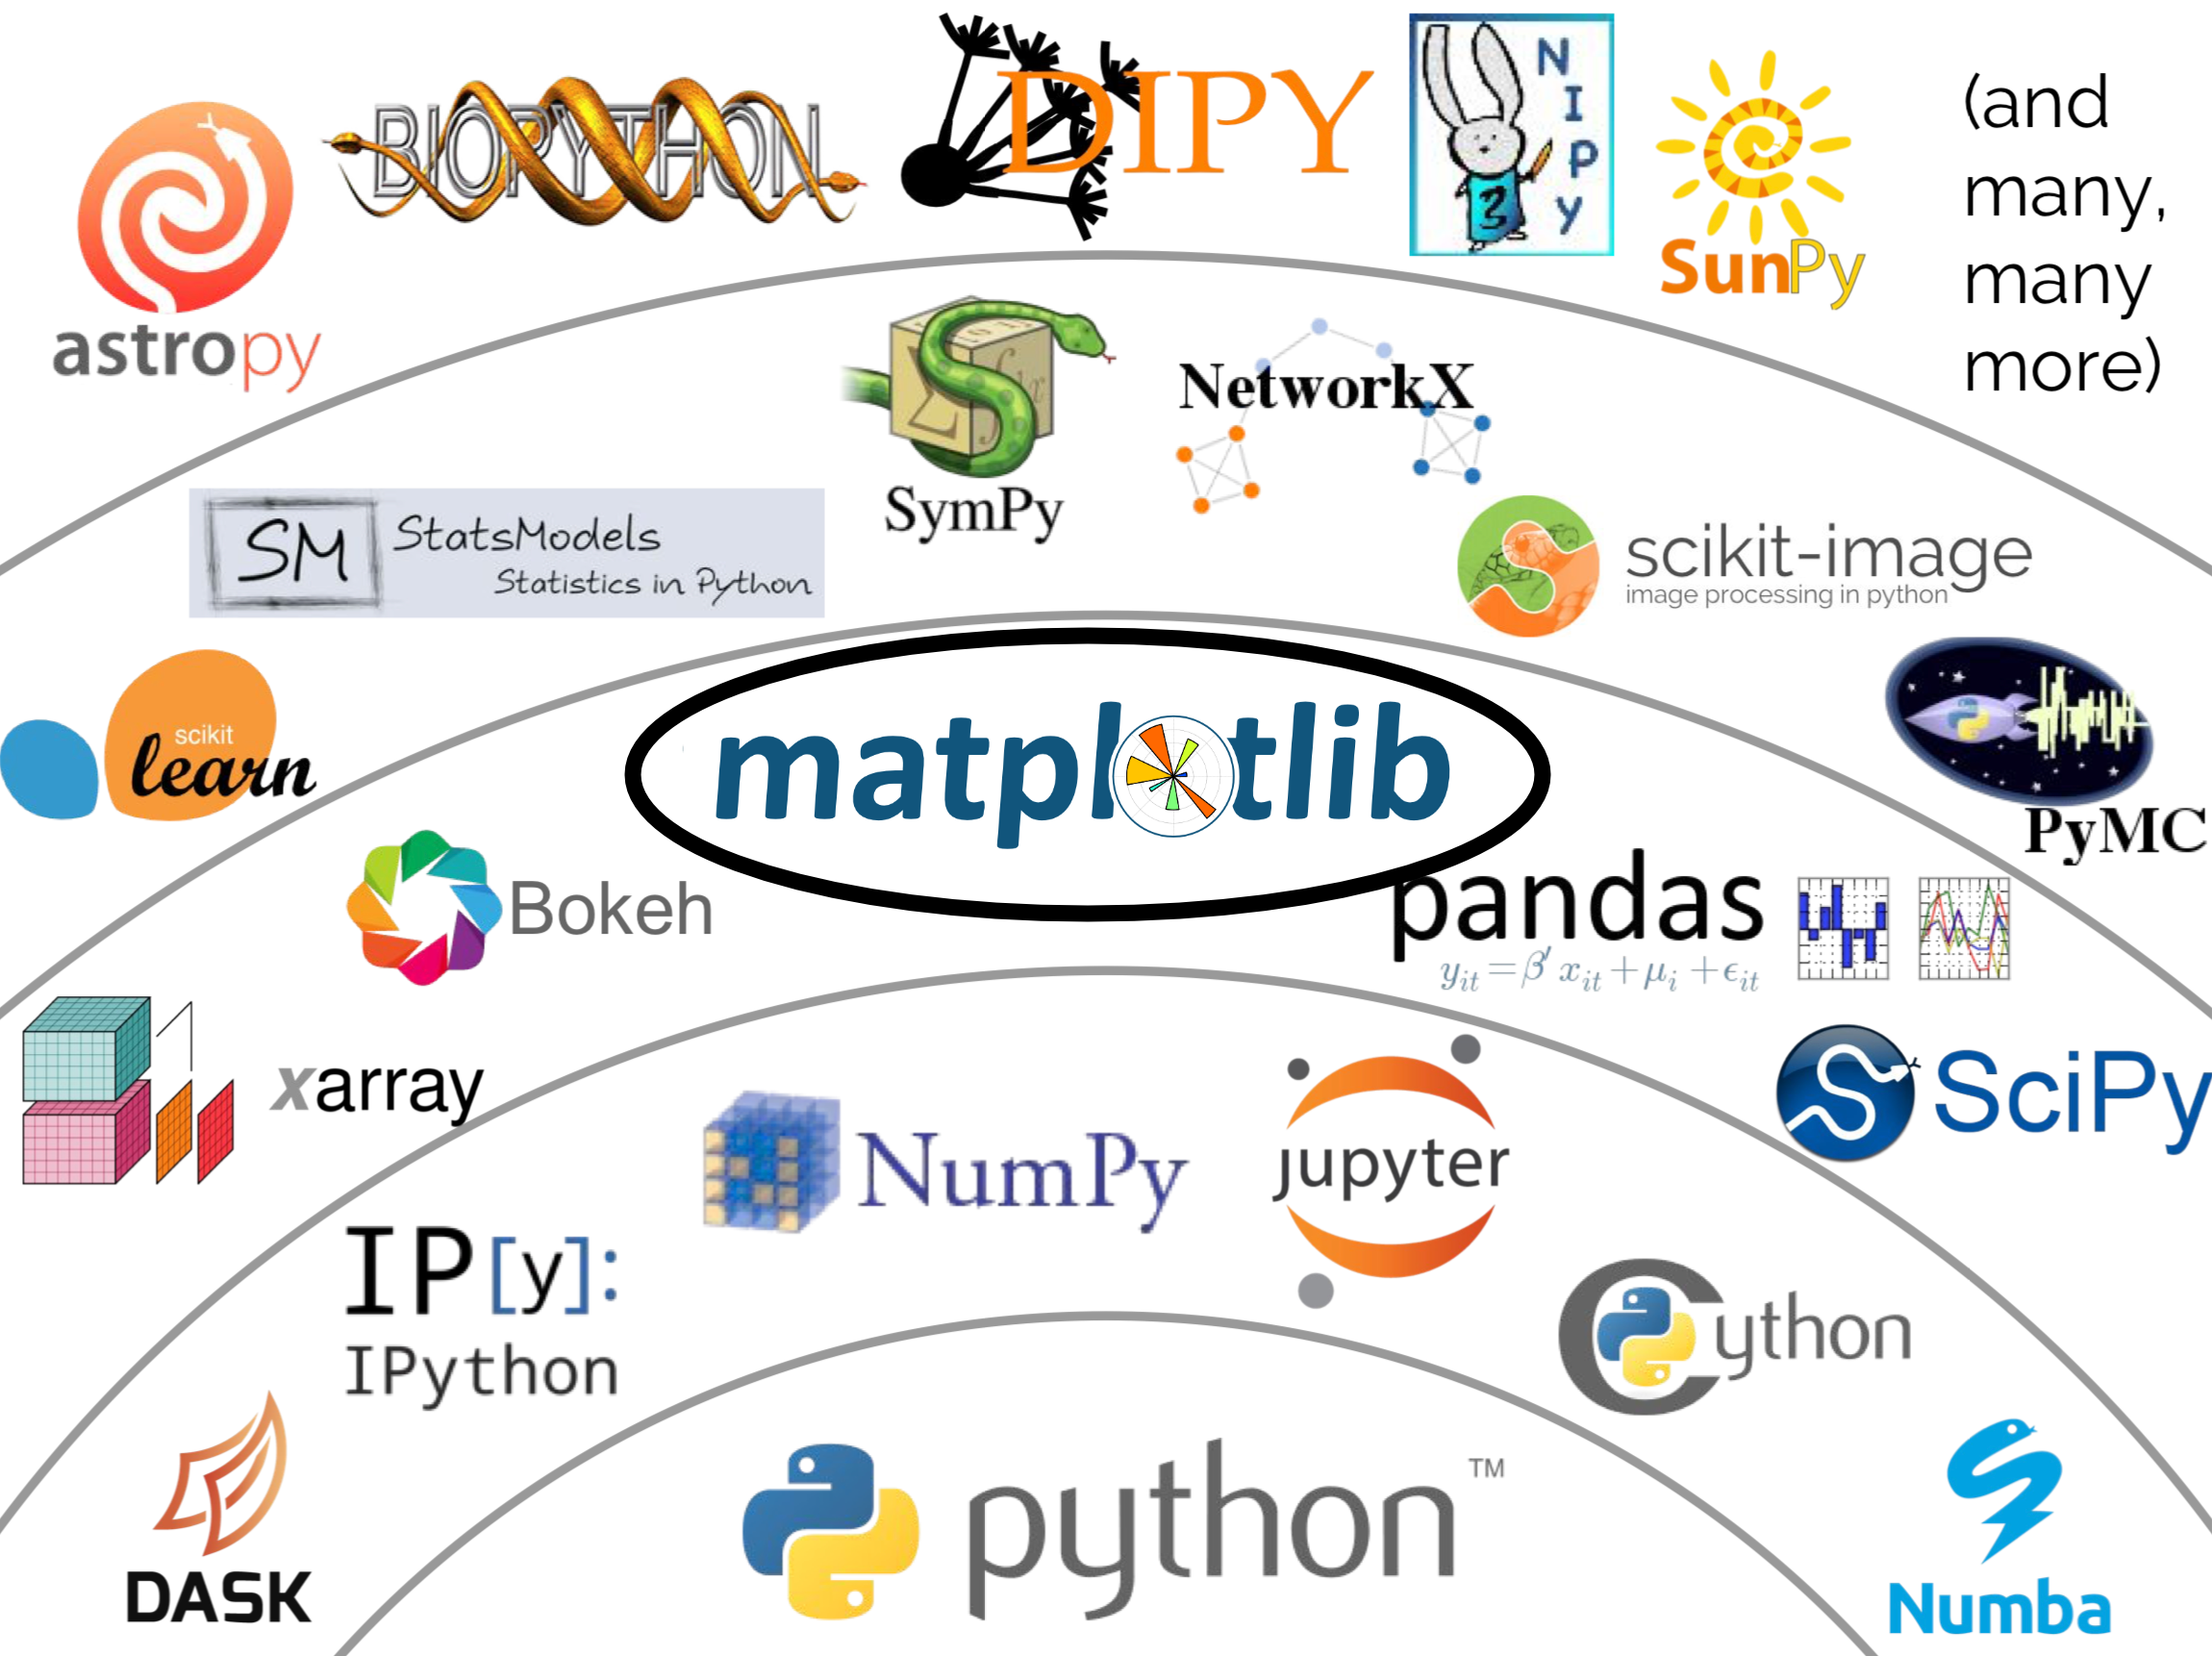
\includegraphics[width=0.45\textwidth]{scipy-ecosystem}
  \caption{A schematic of the Scientific Python ecossytem.  At the
    center we have the Python language itself with concentric rings of
    domain agnostic to domain specific libraries.  Both AstroPy (top
    left) and SunPy (top right), used in the astrophysics and
    heliophysics divisions respectively, rely on Matplotlib.
    Credit: Jake van der Plas, "The Unexpected Effectiveness of Python
    in Science", PyCon 2017}
  \label{fig:ecosystem}
\end{wrapfigure}



Matplotlib~\cite{Hunter:2007} is an established open source plotting
library with a BSD-derived license that is currently used throughout
both the SMD science community and the wider scientific community.
The initial work on Matplotlib was done in 2001-2002 and the first
commits in the Matplotlib history date to early 2003.  Over the last
17 years Matplotlib has been actively developed and maintained by a
vibrant, primarily volunteer, community.  Matplotlib has over 1,250
individual contributors to the code base with countless more
individuals having contributed in ways not easily track, such as
answering user questions on the mailing list or reporting issues.

Matplotlib has a high-level API for quick plotting, such as in
exploratory data analysis, plus a low-level API that gives full control for
fine-tuned publication-quality plots, for animations, for writing both
GUI-independent and GUI-specific tools for interactive data plotting, and
for output to a variety of vector and raster
formats including \texttt{svg}, \texttt{eps},
\texttt{pdf}, and \texttt{png}

Matplotlib APIs as readily extendable.  The most common visualizations
in a domain need to be fluid for the end-practitioners, with the
``obvious'' customization options exposed. Much of the domain-specific
specialization is carried in the structure, semantics and assumptions
of the data, and in the standard visualizations of the domain. These
specializations can vary widely, in contradictory ways, between
domains. Because no high-level API can simultaneously satisfy all of
the visualization needs, there has developed a rich ecosystem of
domain specific plotting tools including yt, astropy, ArviZ,
seaborn, xarray, astropy, fast\_histogram extending the core
Matplotlib APIs.


While large parts of the scientific computing community rely on the
SPE, the open nature of these infrastructure tools makes measuring
their influence hard.  Conservative estimates, based on downloads and
web traffic on the documentation, are that Matplotlib has over a
million users.  We expect that a large fraction of NASA SMD-sponsored
projects rely on this shared infrastructure to some degree, but this
is hard to prove in practice.  In particular, scientific work does not
usually cite the software that was used for computation and plotting,
and usage and download statistics are hard to gather for widely used
open source packages.  Even though citation counts are likely to
vastly under-represent the scientific use of these packages, a
canonical reference for Matplotlib~\cite{Hunter:2007} has over 12,750
citations while a common reference of NumPy~\cite{walt2011numpy} has
over 6,800 citations. These counts already illustrate a problem in
measuring usage via citations, as every user of Matplotlib also uses
NumPy, but Matplotlib has almost twice as many citations.  Domain
specific tools, like AstroPy~\cite{robitaille2013astropy} for
astronomy (about 4,500 citations), often have high citation counts
compared to the core packages like NumPy, SciPy and Matplotlib that
they are built upon.


\subsection{Objectives and Significance}



% - need to re-engineer Matplotlib's data model
% - have on-going work to do design and prototypes
% - need significant SEW effort to implement across whole library
% - one nice thing is units, focus on documenting / planning / testing
% - another nice thing is resampling and out-of-core data access
% - we have to do this while keeping the patient writing papers


Matplotlib is a primarily community-driven project, but we have grown
to the point where we need supported developers with the time to
organize, plan, and make decisions.  Supported developers will allows
us to take on bigger projects than can be implemented by volunteer
effort alone and to ensure that the critical day-to-day maintenance
tasks required to keep the project healthy are done.  We propose to
split the effort on this grant equally between a major development
effort, overhauling our internal data representation, and general
library maintenance.


\subsubsection{Refactor Internal Data Model}

While this elides many implementation details, for the purposes of
this proposal it is sufficient to understand \texttt{Artist}s as the
objects in Matplotlib that, given user data, produce something visible
in the output.  Internally Matplotlib represents a \texttt{Figure} as
a tree of \texttt{Artist}s~\cite{AOSA_mpl}.  Each individual
\texttt{Artist} is responsible for holding the user data and style
information for a part of the final visualization.For example,
\texttt{matplotlib.text.Text} is the class responsible for drawing
text.  It holds, among other things, the location of the text, the
string, and the font, size and color to use.  The plotting methods in
Matplotlib create these objects and add them to the tree.  To render
the final output Matplotlib walks the \texttt{Artist} tree depth-first
and each each \texttt{Artist} is responsible for rendering itself to
output.

Currently, each plotting method and \texttt{Artist} handles sanitizing
and storing data independently.  Hence, some common functionality,
such as handling data with attached units (e.g., degrees Celsius,
dates), is repeated throughout the code base and each \texttt{Artist}
subclass holds its data in a different way.  This leads to
inconsistencies across the library and makes it difficult for users to
write code that updates interactive explorations and animations.
Another consequence is that Matplotlib also cannot exploit
``Structured data''--combining multiple pieces of (possibly
heterogeneous) data with labels and metadata into single data
structure; instead, users must extract data elements and reassemble
them as arguments to Matplotlib plotting functions.

We have on-going theoretical and design work\footnote{Supported by
CZI} to re-architect Matplotlib to better separate the data
representation from the rest of the library.  We are developing a
consistent data access API such that each \texttt{Artist} will have a
single \texttt{DataSource} object responsible for providing access to
all of the data that the \texttt{Artist} needs.  This design will
allow us to over come many of the issues with the current design and
open the door to a variety of new functionality.  The current work is
expected to produce design documents and a proof-of-principal
implementation by the end of 2021.  Based on this preliminary work
\textbf{we propose refactoring all of Matplotlib to use the new data
  model}

One of immediate benefit of the refactoring will be to drastically
improve Matplotlib's handling of data with physical units attached.
Units are fundamental to science and engineering, however most
numerical software is unit-naive.  It is the user's responsibility to
keep track of and correctly convert data to consistent units prior to
any computation.  Failing to do so leads to the most insidious of
bugs: everything ``works'' but silently gives incorrect results!
There are several libraries which provide unit-aware data structures
in Python.  When registered, Matplotlib can use object from these
libraries for unit-aware plotting.  \textbf{This capability it is
  currently used to support spaceflight operations by Monte, JPL's
  mission design and navigation software system} and the initial
development was supported by NASA.

% to what extent mpl currently supports units

The current support physical units in Matplotib is base on type
inference and dispatch of the input.  When the unit-full data is
passed by the user the we look up the converter, default axis label,
limits, and functions for locating and formatting the ticks, to use.
Matplotlib registers converters for datetime and string-categorical
types by default and third-party libraries to register themselves.
Using this machinery users can control what units the data is plotting
in, which may be different than the units it was passed in as, and
specify the limits in physical units.


% what is wrong
However, there are several problems with the current unit support in
Matplotlib.  It is under documented making it difficult for users to
understand and use the capability and for developers to extend.
Coupled with a lack of full test coverage of using physical units,
over time the inconsistencies mentioned above have accumulated in the
code base.  These range from subtle inconsistencies between plotting
methods to unit-full data simply not working with some methods.
\textbf{To address this we propose to use unit-handling as a
  motivating feature while doing the \texttt{DataSource} refactoring}.
By implementing all of the unit logic in the \texttt{DataSource} we
will be able to share the code across all \texttt{Artist}s and unify
how we treat units across the library.


\subsubsection{General maintenance}

To maintain Matplotlib's health we need to:
\begin{itemize}[noitemsep]
\item fix critical bugs and regressions;
\item triage the backlog of Issues and PRs in terms of topic,
  difficulty, and urgency and promptly triage newly opened Issues and
  PRs;
\item maintain backward compatibility and extensively document
  intentional changes;
\item on-board new contributors to sustain and diversify developer
  team;
\item maintain the CI infrastructure;
\item manage the release process;
\item and manage discussions about proposed enhancements, features,
  and API changes.
\end{itemize}
These are tasks that are never ``done''; users find new ways to use
the library expose previously un-detected bugs, request or propose new
features and the world continues to changes around us.  \textbf{While
  this critical work can be done by volunteers, however supported
  developers help ensure that things happen in a timely manner}.

%% sentences that I still like, but don't fit into the flow at all

% Maintenance is inherently reactive, we do not know about new bugs,
% user issues, or breaking changes in upstream packages until they are
% reported gobto us.

% There are a number of tasks that are required to ``keep the lights
% on'' on a Python package include maintaining the continuous
% integration systems, managing releases, tracking down
% platform-specific bugs, and tracking upstream changes.


%plot?

Historically, Pull Requests (PRs) and Issues have been submitted
faster than they can be reviewed; Matplotlib has accumulated about 300
open PRs 1300 open Issues due to this imbalance, There almost
certainly are critical bug reports or insightful feature requests among
the issue backlog, while among the PR backlog there are useful contributions
or bug fixes that would improve the libraries for direct users and
downstream packages.  The large backlog is discouraging for new and
occasional contributors and distracting for core developers.

In 2020 Matplotlib resolved 125-200 PRs and 75-125 Issues a month,
however even at this rate we only reduced the PR backlog by 70 open
PRs and held even on the Issue backlog.  We were able to achieve this
because for 10 months in 2020 we had supported Research Software
Engineer (RSE) working on Matplotlib.  As part of reducing the
backlog, we were able to fix a several long standing bugs.  We have
demonstrated that supporting maintenance work has a positive effect on
the health of the project and \textbf{the additional resources
  requested here will further reduce, but not eliminate, the
  maintenance backlog}.


\subsection{Perceived impact of work}

% TODO add cite for
% \url{https://www.aosabook.org/en/matplotlib.html}

Originally developed over 17 years ago the architecture of Matplotlib
it has served us extremely well, however it does not reflect recent
developments in software design, data structures, and visualization.
Refactoring the data layer will be a major step towards continuing to
support and enable science for the next 20 years.  In addition to fixing
the support of physical units, this refactor will lay the ground work for
\begin{itemize}[noitemsep]
  \item smart down-sampling of plotted data based on view limits,
  \item native consumption of structured data,
  \item seamless updating of the underlying data, either interactively
    or via streams,
  \item and use of alternative data sources such as database queries
    or analytic functions.
\end{itemize}
These features will be increasingly relevant as the scale and complexity
of data continues to increase.


There is a broad recognition across the SPE of the importance of
supporting physical units as an intrinsic component of computation.
There is on going work in NumPy (NEP40-43), pandas, and xarray to add
support for physical units to the foundational data structures.  The
proposed work in Matplotlib will ensure that Matplotlib is ready to
plotting unit-full data to provide users with a complete solution to
working with unit-aware data.

From major projects, like \texttt{yt}, \texttt{CartoPy} or
\texttt{astropy}, to a grad student's experiment-specific plotting
tools users compose the core Matplotilb APIs to fit their unique data
structures and visualization needs.  This extensibility is one of the
key features of Matplotlib and source of its longevity and ubiquity.
Refactoring the data access will open up new paths for users and
down-stream to extend Matplotlib to built highly-tuned domain specific
plotting tools.

Supporting Matplotlib is a highly leveraged investment.  Improvements
to Matplotlib will be seen both directly by our users and by the
developers of tools that depend on Matplotlib and transitively by
their users.  For example, \texttt{Monte} and
\texttt{astropy} are libraries developed and used by SMD researchers
that make use of the unit machinery in Matplotlib.   Improving the
unit handling in Matplotlib will directly improve those libraries.

The library has grown organically over time through the contributions
of over 1,300 individuals, accumulating many small inconsistencies in
the API.  For example, similar methods have different argument order,
e.g., \texttt{ax.text(x, y, s)} vs \texttt{ax.annotation(s, (x, y))},
and some keyword (named) arguments can be singular or plural, e.g.,
\texttt{color} vs \texttt{colors}.  These subtle issues add friction
for users, but are hard to fix without breaking existing code for
someone in our large user base.  While not sufficient to address these
issue, unifying the data representation is a necessary first step.


% \begin{enumerate}
% \item increased reliability of unit-aware plotting
% \item improvement in general reliability of software
% \item improved responsively to issues
% \item making point about building on current funding
% \end{enumerate}
%
% - [x] improving the maturity and sustainability of the project (WC)
% - [x] direct user impact?
% - [ ] what new science?!
% - [x] need to be ``outward looking'' (which should anyone else care?)
% - [x] make stronger point that yt, astropy, monte all use units -> will make their life better
% - [x] helps make the point the mpl is tool for other projects, not end in its self
% - [x] supporting long term goal to make API more consistent and easier to use
% - [x] tie to numpy/panda/xarray dtype work strongly


This proposal is another step towards Matplotlib sustainability.
Given the usage and the scale of the library it is not sustainable to
continue to maintain Matplotlib on majority volunteer effort, which
requested support for developers is intended to complement and
facilitate, not replace.  We aim to better co-ordinate and nurture
volunteer efforts, with the goal of growing and sustaining a diverse
community of volunteer and paid expert contributors.


\subsection{Relevance to program element}

As mentioned above, it is hard to estimate the prevalence of open
source software due to it being freely distribute and not
systematically cited.  Matplotlib is in the top 100 most-downloaded
packages from PyPI~\cite{pypi_stats} and is packaged by every major
Linux and scientific Python distribution.  One path is static analysis
of publicly available code.  According to github over 299K
repositories and over 12k packages hosted on GitHub depend on
Matplotlib~\cite{gh_deps:2021} and a recent study of the almost 10M
Jupyternotebooks on github found that over 3M of them have a
Matplotlib import~\cite{datalore:2020}.


All of these measures show broad impact but cover many uses outside of
the SMD community.  [something about how to restrict static analysis,
  many scientist do not make code public].  Soliciting for examples of
Matplotlib in SMD research on social media yielded a (non-exhaustive)
list of examples of using Matplotlib
\begin{itemize}
\item
  to study
  thunderstorms~\cite{https://doi.org/10.1002/2016JD025299,https://doi.org/10.1029/2019JD030874},
  seasonal ocean winds~\cite{https://doi.org/10.1002/2017JD027516} and
  tropical storms~\cite{Lang_2020};
\item in the first science paper from the Parker Solar
  probe~\cite{Bale2019};
\item in the Martian science program in both
  orbiter~\cite{https://doi.org/10.1029/2019JE006188} and
  rover~\cite{https://doi.org/10.1002/2016EA000219} contexts;
\item as part of ground operations from the Phoenix Lander;
\item with data from Kepler and K2 missions to study Trojan
  asteroids~\cite{Nixon_2019} and
  Titan~\cite{Ryan_2017,2019PASP..131h4505P};
\item on the New Horizons Kuiper belt extended
  mission~\cite{Porter_2018};
\item for visualization of scheduling, safety and constraint checks,
  and telemetry by the Swift science operations
  team~\cite{swift_ops,2020ApJ...900...35T};
\item as port of the Hubble Space Telescope and James Web Space
  Telescope data processing pipelines;
\item in Monte, JPL's mission design
  and navigation software system to support spaceflight operations;
\item in fundamental research on graphene~\cite{PhysRevLett.120.236802};
\item and for work on nuclear rockets~\cite{leu_cerment}.
\end{itemize}
This list shows the breadth of the use of Matplotlib across the
four SMD divisions.  Small investments in Matplotlib will have returns
across the entire SMD portfolio.

\subsection{sources of uncertainty/mitigation to risk}

As show above, Matplotlib is widely used, both directly and
transitively.  Given the large user base it is imperative that changes
are as backwards compatible as possible.  While this large user base
is on one hand a lever that magnifies any improvements, it also makes
changes more expensive.  We can not simply change our public to track
the internal refactoring, instead we must write also write code to
translate the old API to the new implementation.  This engineering work
makes the refactor more challenging and time consuming than starting
from scratch.

% - need to be very careful about not breaking back-compatibility

The biggest risk with the proposed work is that we are underestimating
the amount of work that will be required for data refactor and unit
work.  There is always a risk while refactoring that the scope of work
rapidly snow ball due to unexpected internal dependencies or edge
cases must be accounted for.  In a worst case where we have to abandon
the work we will maintain the status quo, but with significantly
better documentation.

We anticipate that all of the work can be done incrementally and will
be merged to the default branch of Matplotlib throughout the
performance period.  Frequently merging incremental work both reduces
the risk it is also consistent with our standard development process.
Work done under this proposal will not be exempt from review, and many
small PRs are easier to review and merge than a single large PR.
These improvements, both to the code and documentation, will be
released to users as part of our standard bi-yearly release cadence.

There is minimal risk in the maintenance work.  There is large volume
of individually small tasks that need to be addressed: the issue and
PR backlogs.  Any dedicated effort devoted to clearing the backlog
will have a positive impact on the project.  We have demonstrated that
supporting developers for maintenance work is an effective and
efficient use of resources.


\subsection{Contributions of Principle Investigator and Key Personnel}

Dr. Thomas Caswell has the sole individual responsibility for the
direction of this work.  He has extensive experience developing and
maintaining Python libraries for use by scientists.  He has been
involved with Matplotlib from 2012 and had a leadership role in the
project from 2014.  At Brookhaven National Laboratory he is the Lead
architect and developer of the Bluesky Suite, an ecosystem of
co-developed libraries and applications for data acquisition and
management, which is being adopted for beamline operations at
synchrotrons in the US and across the world.



\subsection{Work Plan}

\begin{ganttchart}[
    vgrid,
    title height=1,
    milestone inline label node/.append style={left=5mm},
    x unit=.75cm,
    %inline,
    %expand chart=\textwidth,
    %milestone/.append style={xscale=12*.75cm/\textwidth},
    milestone/.append style={xscale=1},
    bar height=.75,
    bar top shift=.125,
    y unit chart=.75cm,
    y unit title=.75cm]{1}{12}
  \gantttitle{2020}{2}
  \gantttitle{2021}{4}
  \gantttitle{2022}{4}
  \gantttitle{2023}{2}\\
  \gantttitle{Y1}{4}
  \gantttitle{Y2}{4}
  \gantttitle{Y3}{4} \\
  \gantttitlelist[title list options=%
  {var=\y, evaluate=\y as \x%
    using " Q\y "}]{1,...,4}{1} \
\gantttitlelist[title list options=%
  {var=\y, evaluate=\y as \x%
    using " Q\y "}]{1,...,4}{1}
\gantttitlelist[title list options=%
  {var=\y, evaluate=\y as \x%
    using " Q\y "}]{1,...,4}{1} \\
\ganttmilestone{Hire RSE}{1} \ganttnewline
\ganttbar{Document Units (internal)}{1}{2} \ganttnewline
% \ganttbar{Document Units (external)}{2}{3} \ganttnewline
\ganttbar{Planning and Design}{2}{4} \ganttnewline
\ganttmilestone{\texttt{DataSource} API stable}{3} \ganttnewline
\ganttbar{Refactor Data Layer}{4}{12} \ganttnewline
\ganttmilestone{SciPy Talk}{4} \ganttmilestone{}{8} \ganttmilestone{}{12} \ganttnewline
\ganttbar[inline]{General Maintenance (ongoing)}{1}{12} \ganttnewline
\ganttmilestone{Matplotlib Releases}{2} \ganttmilestone{}{4} \ganttmilestone{}{6} \ganttmilestone{}{8} \ganttmilestone{}{10} \ganttmilestone{}{12}
\end{ganttchart}


Starting from July 2021 onward through July 2024 Dr. Caswell will
devote 25\% FTE to this work.  His time will be split between the data
layer refactor, community management, and general maintenance work,
the later two being on-going tasks.  The first critical task will be
the recruitment and hiring of the RSE which should be accomplished by
the end of the first quarter of the work period.

% 4 part plan
%  1. document how units work now, document how it should work, id problems
%  2. work to adapt the theoretical and prototype datasource work to API stable
%  3. plan!
%  4. re-write every Artist sub-class



The first task is to document, both at the conceptual and API level,
how the unit dispatch system currently works in theory and practice.
Given the importance of backwards compatibility it is critical to
understand what we are refactoring before beginning.  This
documentation will be aimed at Matplotlib developers and third-party
library authors and focus on the low-level details.  Unfortunately,
the original authors of the unit-handling code are no longer active
with the project so we may have to reverse engineer some aspects of
the code and motivation.

% Internally we need to convert
% unit-full data to unit-naive values to pass to the next layer down.
% A
% common problem we have seen is issue with when and where we do that
% conversion.
% This documentation will clarify which layer of the API
% the conversions should be done in and how both the converted and
% unconverted data should be tracked and managed.
% For unit-aware
% plotting to be fully useful, it must work in every plotting method,
% thus we need clear documentation so that every Matplotlib developer is
% familiar with how unit works.
% Understanding and documenting how the
% unit-mechanism was intended to work and the current state of the
% library will be the foundation of the rest of the work.


The second task is to write user-facing documentation and tutorials
showing how to work with unit-full data and Matplotlib.  We will document
the expected behavior and API


For this we will work
closely with maintainers of unit libraries, such as \texttt{unyt}
(\url{https://unyt.readthedocs.io/}), \texttt{pint}
(\url{https://pint.readthedocs.io/}) and
\texttt{astropy.units} (\url{https://docs.astropy.org/en/stable/units/}),
and user within the SMD community, such as the Monte developers at JPL
and the Astropy developers, to ensure that we are fully meeting their
needs.

The user documentation will also focus on how things should be
and will serve as a guide for what the ``correct'' behavior is when we
are resolving inconsistencies.  This work will tie into our ongoing
effort to make our large API surface more self-consistent and easier
to use.

\textbf{Implementation}

The third task is to ensure that all of the plotting methods support
unit-full data in a uniform way.  The documentation developed as part
of the first two tasks will guide how we resolve any inconsistencies.
This work will build on ongoing work supported work, funded by Chan
Zuckerberg Initiative, to re-design how we store data internally.
Currently each \texttt{Artist} is responsible for storing its data and
each does it in its own different way.  This variation and duplication
in the implementation is also the source of many of the unit-related
regressions.  The proposed redesign will factor the data storage out
of the \texttt{Artist}s into a reusable class.  Among the benefits of
this design, we will be able to centralize the unit processing and
dispatch to one place in the code.  We expect the design and
proof-of-concept work of this re-design to be complete by the end of
2021 which aligns with the period of work of this proposal.  Building
on the data source work, we propose implementing this new design in
all \texttt{Artist} subclasses, any required changes to the plotting
methods, and adding full test coverage of unit handling in every
plotting method.  This work will require touching and testing a large
fraction of the library.

- [TODO] makes future mpl development easier by documenting and simplifying
  the internal handling of units
- make sure it fits with new numpy dtype scheme (NEP 40-43)
- make sure it works with pandas dtypes?

A final task is to extend the unit machinery to improve the user
experience.  Currently much of the mechanism of unit-handling is
implicit and automatic based on type inference.  We propose to extend
the interface to allow optional direct control of the unit machinery
by users and third-party library developers.  We will rely on the
documentation and testing from the previous work to ensure that we do
not introduce any new regressions or inconsistencies.



The Research Software Engineer (RSE), whom needs to be identified,
will devote 100\% FTE to this project.  This will be split evenly with
50\% FTE being spent on the unit work and 50\% being spent on general
maintenance until the unit work is complete.  If the unit work is
completed faster than expected, the RSE will devote 100\% of their
effort to maintenance.  Because Matplotlib is a community project, the
work of the RSE will still go through the normal review process.  The
interaction with community makes it advantageous to spread out the
unit work.  The first task, producing developer-facing documentation
about how the unit system works we expect to take 25\% FTE with will
be spread across the first two quarters of the grant.  Similarly,
writing the user-facing documentation should take about 25\% FTE which
will be done is the third and forth quarters of the performance
period.  The remaining work on units, adding the tests, fixing any
bugs and inconsistencies, and any required internal refactoring, will
take 1 FTE spread across final 2 years of the performance period.
Incremental progress will be merged and released as part of the normal
release cycle throughout the performance period.  The RSE will present
the status of the work at two conferences, expected to be SciPy in
July and one of PyData conferences in the winter, yearly.




\subsubsection{Grant Management Plan}

Dr. Caswell of BNL is the PI of the proposed development and is the
Matplotlib Lead Developer.  He is solely responsible for the quality
and direction of the proposed work and the proper use of all awarded
funds.  He is also responsible for all management, and budget issues
and is the final authority for this task.


\subsection{Project Management}
\subsubsection{Governance}
Matplotlib is a NumFOCUS Fiscally Sponsored Project.  The governance
is specified at
\url{https://github.com/matplotlib/governance/blob/master/governance.md}.
The project has a Project Lead (Caswell) who is the final authority in
all decisions, however when possible all decisions are made by
community consensus.  In addition to the Project Lead, there is a
formalized Steering Council which is responsible for the overall
direction of the project, and several Deputy Project Leads who have
day-to-day technical responsibilities.

TODO need to cover history of project lead changing

\subsubsection{License}

BSD-derived

\subsubsection{sustainability metrics}
\begin{enumerate}
\item Continue Regular releases (mpl minor every 6mo, patch every 2mo
  or as needed).
\item Increase number of new regular contributors
\item Rate of PR / Issue throughput
  \begin{enumerate}
  \item caveats on how issues/PRs are very varied in time to resolve
  \end{enumerate}
\end{enumerate}

\subsubsection{collaboration with related projects}

None of the projects in the Scientific Python ecosystem existing in a
vacuum; a vast majority of our users use more than one of the
projects.  In a mirror of that, while developer communities exist
around each of the code bases, there is also a broader developer
community across the projects.  Matplotlib developers are part of this
community and have well established relationships with the other
projects in the ecosystem, including our key up and down stream
dependencies.

Much of the communication is through the standard communication
channels, such as project issue trackers, mailing lists or discussions
forums, and submitting PRs.  The strongest relationships, both
historical and current, are with projects where we have shared
developers.  For example Ryan May and Elliot sales de Andre are both
core contributors to Matplotlib and Cartopy and David Stansby is a
maintainer on both Matplotlib and \texttt{SunPy}.  Micheal Droettboom,
the previous Matplotlib Project lead, was a core developer on Astropy.
Additionally, through NumFOCUS and domain-specific conferences there
are regular in-person meetings.

[TODO not sure where this fits?] Almost all of the Matplotlib
contributors, are domain experts in their primary domain and use
Matplotlib for their research.


% wording all NF projects are putting in, please avoid wordsmithing it.
As a NumFOCUS project, we recognize the importance of every project
that is part of our open source scientific computing community. Though
we would like for our work to be funded we are committed to supporting
and collaborating with other NumFOCUS projects that receive funding
regardless of our own outcome. We believe that this attitude is
crucial for the success of our community and the sustainability of
open source projects. It is our hope that this sentiment will be taken
into consideration when evaluating our proposal.


\subsubsection{inclusive practices}

Matplotlib strives to be an inclusive and open project and have
adopted a Code of Conduct
\url{https://github.com/matplotlib/matplotlib/blob/master/CODE_OF_CONDUCT.md}. Anyone
who is willing and able to contribute to the project should feel
welcome to do so.  It is important for everyone working on the project
to feel safe to make mistakes.

We have recently started two efforts to improve the development and
retention of new contributors: an ``incubator'' channel on gitter and
a Triage Team.

The hardest part of getting started to contributing to open source
projects is can be simply getting started.  The incubator is a
semi-closed chat room where new contributors can get support on any
aspect of contributing to Matplotlib.  This include the technical
aspects of the code they are working on, help with git/github, our
review process, or the social expectations and norms of the community.  The
goal is that by providing this support to first time contributors we will
retain more of them as regular contributors and then maintainers.

The issue tracker is important to communication in the project because
it serves as the centralized location for making feature requests,
reporting bugs, identifying major projects to work on, and discussing
priorities.  For this reason, it is important to curate the issue
list, adding labels to issues and closing issues that are resolved or
unresolvable. Triaging issues does not require any particular
expertise in the internals of Matplotlib but is extremely valuable to
the project.  To this end we have created a ``Triage Team'' in the
organization who have power to tag, milestone, and close issues.  In
addition to the direct benefit of improving the issue triage and
freeing the core-developers to spend more time reviewing PRs, this
role will bring more people into the developer community and may
provide a path way to becoming regular contributors and maintainers.

One challenge of being an open community developed project is that we
do not have reliable demographics on a vast majority of our
contributors.  Ongoing work at NumFOCUS to develop metrics will help
us evaluate the efficacy of these efforts at diversifying our
contributor base.

\subsubsection{information dissemination}

As a project Matplotlib maintains a range of communication channels
aimed at several, overlapping, audiences.  This includes a
the source, issue tracker and PRs on GitHub,
the published documentation (inculding historical and ``future'' versions),
weekly developer call,
mailing lists,
a discourse forum,
an active chat room on gitter,

in-person presentations at conferences and pydata events,
a blog, and several social media accounts.


The center of gravity of Matplotlib development takes place on GitHub
(\url{https://github.com/matplotlib/matplotlib}) where the canonical
repository for the source and documentation are hosted.  Around this
repository we use Issues and PRs to track bug reports, feature
requests, and to discuss proposed changes.  We also host our
governance documents on GitHub
(\url{https://github.com/matplotlib/governance}) and revise them via
Pull Request.

We publish extensive prose, example, and API documentation
(\url{https://matplotilb.org}) that is refreshed with each release.
In addition to the top-level docs, which always refer to the most
recent release, we also host historical
(\url{https://matplotilb.org/3.1.3} for the v3.1.3 documentation) and
development versions of the documentation
(\url{https://dev.matplotilb.org}).  In 2020 we had between 700k-1M
unique visitors a month to the documentation.


The weekly developer calls are typically attended by six to eight
people and are used for high-bandwidth discussions about both the
overall direction of the project and technical issues depending on the
day.  The agenda and minutes are publicly available
(\url{https://hackmd.io/team/matplotlib}) and the calls are open to
all.

Matplotlib has an active gitter
(\url{https://gitter.im/matplotlib/matplotlib}) chat room.  Gitter is
a real-time chat platform that we use for general coordination and
resolving minor technical discussions.  While the chat room's history
is technically persistent, we treat it as transient.  For more in
depth discussions or anything we want a record of, we move the
conversation to github, the mailing list, or discourse.

For user support and general discussion we maintain two mailing lists,
matplotlib-users
(\url{https://mail.python.org/mailman/listinfo/matplotlib-users}) for
user support and matplotlib-devel
(\url{https://mail.python.org/mailman/listinfo/matplotlib-devel}) for
developer discussion and announcements, and a discourse
(\url{https://discourse.matplotlib.org}) instance.  While users have
to subscribe and register respectively to post, these forums are open
to all.  We also maintain a read-only mailing list for announcements
(\url{https://mail.python.org/mailman/listinfo/matplotlib-announce}).

When we could travel Matplotlib developers would frequently attend
in-person meetings including SciPy and PyData events.

We have a blog (\url{https://matplotlib.org/matplotblog/}) which hosts
user-submitted content highlighting work they have done using
Matplotlib.  We have project accounts on several social media platform
including twitter and Instagram.


\subsection{current workflow}
%check that this is not a required title
%\subsection{Technical approach and methodology}


Matplotlib is an established community driven project in the
``federation'' model as defined by Nadia Eghbal~\cite{eghbal_2020}.  We
have a core group regular maintainers who take responsibility for
reviewing and merging proposed changes to the library.  We strive for
consensus and rely on the collective judgment of our maintainers to maintain
the quality and functionality of the library.

Matplotlib uses a variation on the ``git flow'' process
(\url{https://guides.github.com/introduction/flow/}) to manage
proposing and reviewing contributions to the library and documentation
though on GitHub
(\url{https://matplotlib.org/devel/coding_guide.html}).  A
contributor, a core maintainer, a regular contributor, or a first time
contributor, proposes a change by opening a ``Pull Request'' from
their fork of Matplotlib.  The proposed changes are reviewed by
maintainers who either request changes, which starts a cycle of
iteration with the contributor, or approve.  In addition to human
review we have an extensive test suite that is automatically run via
cloud services and the results are reported to the PR.  Once consensus
is reached and the test pass the PR is merged and the changes will be
released as part of the next release.

The threshold for merging a PR depends on the reviewer judgment of the
risk of the changes.  PRs that only change documentation, which cannot
introduce regressions or introduce new features, may be merged by the
first reviewer where as code changes need to be reviewed and approved
by at least two maintainers.  However in either case a maintainer may
wish to leave a positive review but not merge the PR to request
additional feed back from other maintainers.  If a maintainer objects
to a PR, the PR will not be merged until their concerns have been
addressed.  If consensus cannot, the final decision falls back to a
Deputy Project Lead or the Project Lead.

Matplotlib is cautious about making backwards-incompatible change that
intentionally break users existing code.  While in an ideal world,
future versions of the library would be 100\% backwards compatible
with previous versions, sometimes we do need to make incompatible
changes.  As part of the review process we check that any API changes
are well documented and justified.  When technically possible we
provide user-visible warnings the version before we actually implement
a breaking change.  This provides a window for users to either adapt
to the change or to communicate to us that they cannot adapt so we
can reconsider the change.  Given this high barrier to changing or
removing behavior we are careful to make sure that any new API we add
to the library is well thought out and complete because once we have
released a version of the library with that code it is hard to take it
back.  These considerations together are important enough that we have
a Deputy Project Lead responsible for API consistency.

This process works well for incremental contributions and bug fixes,
new features or bigger changes are typically discussed before
significant work is done.  In many cases if the feature does not need
to be in the core library we encourage contributors to create a new
stand-alone project.  This has several advantages including the giving
the author more control, allows them to iterate faster than our
relatively slow 6 month release schedule, and gives them greater
flexibility to change their APIs.


\newpage
% Here's how I get references.
% needed for AAS citation

\def\ref@jnl#1{{\rm#1}}

\def\aj{\ref@jnl{AJ}}                   % Astronomical Journal
\def\actaa{\ref@jnl{Acta Astron.}}      % Acta Astronomica
\def\araa{\ref@jnl{ARA\&A}}             % Annual Review of Astron and Astrophys
\def\apj{\ref@jnl{ApJ}}                 % Astrophysical Journal
\def\apjl{\ref@jnl{ApJ}}                % Astrophysical Journal, Letters
\def\apjs{\ref@jnl{ApJS}}               % Astrophysical Journal, Supplement
\def\ao{\ref@jnl{Appl.~Opt.}}           % Applied Optics
\def\apss{\ref@jnl{Ap\&SS}}             % Astrophysics and Space Science
\def\aap{\ref@jnl{A\&A}}                % Astronomy and Astrophysics
\def\aapr{\ref@jnl{A\&A~Rev.}}          % Astronomy and Astrophysics Reviews
\def\aaps{\ref@jnl{A\&AS}}              % Astronomy and Astrophysics, Supplement
\def\azh{\ref@jnl{AZh}}                 % Astronomicheskii Zhurnal
\def\baas{\ref@jnl{BAAS}}               % Bulletin of the AAS
\def\bac{\ref@jnl{Bull. astr. Inst. Czechosl.}}
                % Bulletin of the Astronomical Institutes of Czechoslovakia
\def\caa{\ref@jnl{Chinese Astron. Astrophys.}}
                % Chinese Astronomy and Astrophysics
\def\cjaa{\ref@jnl{Chinese J. Astron. Astrophys.}}
                % Chinese Journal of Astronomy and Astrophysics
\def\icarus{\ref@jnl{Icarus}}           % Icarus
\def\jcap{\ref@jnl{J. Cosmology Astropart. Phys.}}
                % Journal of Cosmology and Astroparticle Physics
\def\jrasc{\ref@jnl{JRASC}}             % Journal of the RAS of Canada
\def\memras{\ref@jnl{MmRAS}}            % Memoirs of the RAS
\def\mnras{\ref@jnl{MNRAS}}             % Monthly Notices of the RAS
\def\na{\ref@jnl{New A}}                % New Astronomy
\def\nar{\ref@jnl{New A Rev.}}          % New Astronomy Review
\def\pra{\ref@jnl{Phys.~Rev.~A}}        % Physical Review A: General Physics
\def\prb{\ref@jnl{Phys.~Rev.~B}}        % Physical Review B: Solid State
\def\prc{\ref@jnl{Phys.~Rev.~C}}        % Physical Review C
\def\prd{\ref@jnl{Phys.~Rev.~D}}        % Physical Review D
\def\pre{\ref@jnl{Phys.~Rev.~E}}        % Physical Review E
\def\prl{\ref@jnl{Phys.~Rev.~Lett.}}    % Physical Review Letters
\def\pasa{\ref@jnl{PASA}}               % Publications of the Astron. Soc. of Australia
\def\pasp{\ref@jnl{PASP}}               % Publications of the ASP
\def\pasj{\ref@jnl{PASJ}}               % Publications of the ASJ
\def\rmxaa{\ref@jnl{Rev. Mexicana Astron. Astrofis.}}%
                % Revista Mexicana de Astronomia y Astrofisica
\def\qjras{\ref@jnl{QJRAS}}             % Quarterly Journal of the RAS
\def\skytel{\ref@jnl{S\&T}}             % Sky and Telescope
\def\solphys{\ref@jnl{Sol.~Phys.}}      % Solar Physics
\def\sovast{\ref@jnl{Soviet~Ast.}}      % Soviet Astronomy
\def\ssr{\ref@jnl{Space~Sci.~Rev.}}     % Space Science Reviews
\def\zap{\ref@jnl{ZAp}}                 % Zeitschrift fuer Astrophysik
\def\nat{\ref@jnl{Nature}}              % Nature
\def\iaucirc{\ref@jnl{IAU~Circ.}}       % IAU Cirulars
\def\aplett{\ref@jnl{Astrophys.~Lett.}} % Astrophysics Letters
\def\apspr{\ref@jnl{Astrophys.~Space~Phys.~Res.}}
                % Astrophysics Space Physics Research
\def\bain{\ref@jnl{Bull.~Astron.~Inst.~Netherlands}}
                % Bulletin Astronomical Institute of the Netherlands
\def\fcp{\ref@jnl{Fund.~Cosmic~Phys.}}  % Fundamental Cosmic Physics
\def\gca{\ref@jnl{Geochim.~Cosmochim.~Acta}}   % Geochimica Cosmochimica Acta
\def\grl{\ref@jnl{Geophys.~Res.~Lett.}} % Geophysics Research Letters
\def\jcp{\ref@jnl{J.~Chem.~Phys.}}      % Journal of Chemical Physics
\def\jgr{\ref@jnl{J.~Geophys.~Res.}}    % Journal of Geophysics Research
\def\jqsrt{\ref@jnl{J.~Quant.~Spec.~Radiat.~Transf.}}
                % Journal of Quantitiative Spectroscopy and Radiative Transfer
\def\memsai{\ref@jnl{Mem.~Soc.~Astron.~Italiana}}
                % Mem. Societa Astronomica Italiana
\def\nphysa{\ref@jnl{Nucl.~Phys.~A}}   % Nuclear Physics A
\def\physrep{\ref@jnl{Phys.~Rep.}}   % Physics Reports
\def\physscr{\ref@jnl{Phys.~Scr}}   % Physica Scripta
\def\planss{\ref@jnl{Planet.~Space~Sci.}}   % Planetary Space Science
\def\procspie{\ref@jnl{Proc.~SPIE}}   % Proceedings of the SPIE

\let\astap=\aap
\let\apjlett=\apjl
\let\apjsupp=\apjs
\let\applopt=\ao
\setcounter{page}{1}
\bibliography{mpl_cartopy.bib}

\newpage
\section{Data Management Plan}
\setcounter{page}{1}

Matplotlib is a software library and does not produce any scientific
data as defined in E.1.2 that needs to be preserved.

Matplotlib is currently developed in the open on GitHub and is
released under a permissive license (the Matplotlib license which is a
derivative of the PSF license and compatible with BSD-3).  All work
done on Matplotlib as part of this grant will be done through the
current workflow, will be publicly available, and released under the
same license.  Matplotlib uses git for version control, thus every
developer has the full history on their computer which provides
significant redundancy.  Tagged releases of the software are published
to PyPI (in both source and binary forms).  In addition, Anaconada,
macports, homebrew, and all major Linux distributions independently
build, package, and host Matplotlib.  User facing documentation is built
and hosted at \url{https://matplotlib.org}.

%do we need something about shape files / map tiles?

Any new libraries created as part of the ROSES award will be developed
in the open on GitHub and will released under a BSD-3 license.

% do we need this?
Any incidental work on other software packages, either upstream or
downstream of Matplotlib, will have to follow the license and
development of process of those projects.


\newpage
\section{Biographical Sketch}
\setcounter{page}{1}
\begin{center}
  \textbf{Thomas A Caswell}\\
  Computational Scientist\\
  Brookhaven National Laboratory\\
  Building 741 P.O. Box 5000\\
  Upton, NY 11973-5000\\
  (631) 344-3146\\
\end{center}

\subsubsection*{Relevant Experience}
13+ years working in data intensive experimental science.  8 years of
experience contributing to Scientific Python, 6 years in leadership
roles.  Current Project lead on Matplotlib, past release manager for
h5py, have contributed to NumPy, Pandas, SciPy, and IPython.
Co-developed \texttt{trackpy}, now widely used in soft-matter physics
community.  Lead architect and developer of Bluesky Suite for data
acquisition now being adopted at x-ray facilities around the world.

\subsubsection*{Education}
Ph.D., Physics, University of Chicago \hfill 2014\\
M.S., Physics, University of Chicago \hfill 2008\\
B.A., Physics, Mathematics, Cornell University \hfill 2007

\subsubsection*{Professional Experience}
Brookhaven National Laboratory, Computational Scientist \hfill 2020 - Present\\
Columbia University, Visiting Associate Research Scientist \hfill 2019 - Present \\
Brookhaven National Laboratory, Associate Computational Scientist \hfill 2017 - 2020\\
Matplotlib Project Lead \hfill 2016 - Present\\
Brookhaven National Laboratory, Assistant Computational Scientist \hfill 2015 - 2017\\
Matplotlib Project Co-Lead \hfill 2014 - 2016\\
Brookhaven National Laboratory, Research Associate \hfill 2014 - 2015\\

\subsubsection*{Honors/Awards (selected)}
Brookhaven National Laboratory Spotlight  Award \hfill 2018\\
Brookhaven National Laboratory Lab Award \hfill 2017\\
Google Open Source Peer Bonus \hfill 2017

\subsubsection*{Refereed Publications (selected)}

\begin{enumerate}[noitemsep]
    \item Rakitin et al. \textbf{Introduction of the Sirepo-Bluesky
    interface and its application to the optimization problems}
    Proc. SPIE 11493, Advances in Computational Methods for X-Ray
    Optics V, 1149311 (21 August 2020)
  \item Allan et al. \textbf{Bluesky's Ahead: A Multi-Facility
    Collaboration for an a la Carte Software Project for Data
    Acquisition and Management}, Synchrotron Radiation News (2019)

  \item Koerner et al. \textbf{A Python Instrument Control and Data
    Acquisition Suite for Reproducible Research}, IEEE Transactions on
    Instrumentation and Measurement (2019)

  \item Tafliovic et al. \textbf{Teaching Software Engineering with
    Free Open Source Software Development: An Experience Report},
    Proceedings of the 52nd Hawaii International Conference on System
    Sciences (2019)

  \item Rumaiz et al. \textbf{Multi-Element Germanium Detectors with
    Integrated Readouts}, Synchrotron Radiation News (2018)

  \item Pandolfi et al. \textbf{Xi-cam: a versatile interface for data
    visualization and analysis}, Journal of Synchrotron Radiation
    (2018). 25, 1261-1270

  \item Chubar et al. \textbf{Spectrum-based alignment of in-Vacuum
    Undulators in a Low-Emittance storage ring}, Synchrotron Radiation
    News (2018)


  \item Rumaiz et al. \textbf{Multi-element germanium detectors for
    synchrotron applications}, Journal of Instrumentation (2018) 13
    (04), C04030

  \item Billinge et al. \textbf{Robust Nanostructure from High
    Throughput Powder Diffraction Data} (2017) Microscopy and
    Microanalysis 23 (S1), 172-173

  \item Arkilic et al. \textbf{Towards Integrated Facility-Wide Data
    Acquisition and Analysis at NSLS-II}, Synchrotron Radiation
    News (2017)

  \item Chubar et al. \textbf{Analysis and Correction of in-Vacuum
    Undulator Misalignment Effects in a Storage Ring Synchrotron
    Radiation Source} (2017) in \emph{Proc. 8th Int. Particle
    Accelerator Conf. (IPAC'17)}

  \item Sammeera K. Abeykoon, et. al, \textbf{Software Tools for X-ray
    Photon Correlation and X-ray Speckle Visibility Spectroscopy}
    NYSDS 2016, IEEE conference proceedings (2016)

  \item Thomas A Caswell. \textbf{Dynamics of the vapor layer below a
    Leidenfrost drop}, PRE 90, 013014 (2014)

  \item Arkilic et al. \textbf{Filestore: A File Management Tool for
    NSLS-II Beamlines}, (2015) in \emph{Proceedings of ICALEPCS2015}

  \item Arkilic et al. \textbf{Metadatastore: A Primary Data Store for
    NSLS-II Beamlines}, (2015) in \emph{Proceedings of ICALEPCS2015}

  \item Thomas A Caswell et al. \textbf{Observation and
    Characterization of the Vestige of the Jamming Transition in a
    Thermal 3D System}, PRE 87, 012303 (2013)
    % , Zexin Zhang, Margaret L Gardel, and Sidney R Nagel

  \item Thomas A Caswell et al. \textbf{A High Speed Area
    Detector for Novel Imaging Techniques in a Scanning Transmission
    Electron Microscope} Ultramicroscopy 109, 304-311 (2009)
    %, Peter Ercius, Mark W Tate, Alper  Ercan, Sol M Gruner, David A Muller.

  \item Thomas A Caswell \textbf{Study and Testing of a Pixel
    Array Detector for Electron Microscope Applications} Cornell
  University Senior Thesis, 2007

  \item Liu et al. \textbf{Quantitative Characterization of Near-Field Fuel
    Sprays by Multi-Orifice Direct Injection Using Ultrafast X-ray Tomography Technique}.
  Society of Automotive Engineers (SAE) Technical Paper 2006-01-1041

\end{enumerate}

\newpage
\section{Table of Personnel and Work Effort}
\setcounter{page}{1}

\begin{tabular}{|l|l|c|c|c|c|}
  \hline
  \multicolumn{6}{|c|}{\cellcolor{gray!30}\textbf{Work Efforts to be Funded by this Proposal}}\\
  \hline
  \cellcolor{gray!30} &  \cellcolor{gray!30}&\multicolumn{4}{c|}{\cellcolor{gray!30}\textbf{Commitment (FTE)}} \\
  \hhline{|*2{>{\arrayrulecolor{gray!30}}-}*4{>{\arrayrulecolor{black}}-}|}
  \cellcolor{gray!30}\textbf{Name }& \cellcolor{gray!30}\textbf{Role} & \cellcolor{gray!30}\textbf{Y1} & \cellcolor{gray!30}\textbf{Y2} & \cellcolor{gray!30}\textbf{Y3} & \cellcolor{gray!30}\textbf{Total}     \\  \hline
  Dr. Thomas A Caswell & Principle Investigator & 0.25 & 0.25 & 0.25 & 0.75 \\  \hline
  -- & Research Software Engineer & 1.00 & 1.00 & 1.00 & 3.00 \\  \hline
  \multicolumn{2}{|l|}{\textbf{Total Funded Work Effort}} & \textbf{1.25} & \textbf{1.25} & \textbf{1.25}& \textbf{3.75}\\    \hline
  \multicolumn{6}{|c|}{\cellcolor{gray!30}\textbf{Work Efforts Proposed, but NOT to be Funded by this Proposal}}\\  \hline
  \cellcolor{gray!30} &  \cellcolor{gray!30}&\multicolumn{4}{c|}{\cellcolor{gray!30}\textbf{Commitment (FTE)}} \\
  \hhline{|*2{>{\arrayrulecolor{gray!30}}-}*4{>{\arrayrulecolor{black}}-}|}
  \cellcolor{gray!30}\textbf{Name }& \cellcolor{gray!30}\textbf{Role} & \cellcolor{gray!30}\textbf{Y1} & \cellcolor{gray!30}\textbf{Y2} & \cellcolor{gray!30}\textbf{Y3} & \cellcolor{gray!30}\textbf{Total}     \\  \hline
  Dr. Thomas A Caswell & Principle Investigator & 0.00 & 0.00 & 0.00 & 0.00 \\  \hline
  - & Research Software Engineer & 0.00 & 0.00 & 0.00 & 0.00 \\  \hline
  \multicolumn{2}{|l|}{\textbf{Total Unfunded Work Effort}} & \textbf{0.00} & \textbf{0.00} & \textbf{0.00}& \textbf{0.00}\\\hline
  \multicolumn{6}{|c|}{\cellcolor{gray!30}\textbf{TOTAL Work Efforts Proposed (Funded + Unfunded)}}\\  \hline
  \cellcolor{gray!30} &  \cellcolor{gray!30}&\multicolumn{4}{c|}{\cellcolor{gray!30}\textbf{Commitment (FTE)}} \\\hhline{|*2{>{\arrayrulecolor{gray!30}}-}*4{>{\arrayrulecolor{black}}-}|}
  \cellcolor{gray!30}\textbf{Name }& \cellcolor{gray!30}\textbf{Role} & \cellcolor{gray!30}\textbf{Y1} & \cellcolor{gray!30}\textbf{Y2} & \cellcolor{gray!30}\textbf{Y3} & \cellcolor{gray!30}\textbf{Total}     \\      \hline
  Dr. Thomas A Caswell & Principle Investigator & 0.25 & 0.25 & 0.25 & 0.75 \\  \hline
  -- & Research Software Engineer & 1.00 & 1.00 & 1.00 & 3.00 \\  \hline
  \multicolumn{2}{|l|}{\textbf{Grand Total of Work Efforts}} & \textbf{1.25} & \textbf{1.25} & \textbf{1.25}& \textbf{3.75}\\  \hline
\end{tabular}



\newpage
\section{Current and Pending Support}
\setcounter{page}{1}
\subsection{Current Awards}
Dr. Caswell is fully supported by NSLS-II operations by the Department of
of Energy.  He has an agreement to reduce time allocated to NSLS-II operations by
the amount of time that is required by this proposal.\\
\begin{tabular}{|>{\raggedright\arraybackslash}p{3.1cm}|>{\raggedright\arraybackslash}p{3.1cm}|>{\raggedright\arraybackslash}p{3.1cm}|>{\centering\arraybackslash}p{2.54cm}|>{\centering\arraybackslash}p{2.54cm}|}
  \hline
   \multicolumn{1}{|>{\centering\arraybackslash}p{3.1cm}|}{\small\cellcolor{gray!30}\textbf{Name of Principal Investigator on Award}}
  & \multicolumn{1}{>{\centering\arraybackslash}p{3.1cm}|}{\small\cellcolor{gray!30}\textbf{Award / Project Title}}
  & \multicolumn{1}{>{\centering\arraybackslash}p{3.1cm}|}{\small\cellcolor{gray!30}\textbf{Program Name / Sponsoring Agency / Point of Contact telephone and email}}
  & \multicolumn{1}{>{\centering\arraybackslash}p{2.54cm}|}{\small\cellcolor{gray!30}\textbf{Period of Performance}}
  & \multicolumn{1}{>{\centering\arraybackslash}p{2.54cm}|}{\small\cellcolor{gray!30}\textbf{Commitment (Person-Month per Year)}}
   \\\hline
     {\small Thomas Caswell} &
     {\small Matplotlib - Foundation of Scientific Visualization (EOSS3)} &
     {\small\raggedright Essential Open Source Software for Science (Cycle 3)\\ Chan Zuckerberg Initiative \\ Dario Taraborelli \\ XXX-YYYY \\ dario@...com}  &
     {\small 01/21 - 01/22} &
     {\small 4}\\
   \hline
\end{tabular}
\subsection{Current Awards}
None

\newpage
\section{Budget Justification}
\setcounter{page}{1}

Due to being an established community driven project most regular
contributors have established and distinct primary institutions.  For
this reason significant portions of the budget will need to be
subcontracted to the primary institutions of key individuals who are
uniquely qualified for this work.

Salary support is requested for PI Thomas Caswell (0.25 FTE in years
1-3).  He will oversee the Matplotlib aspects of the proposed work and
co-supervise the RSE.

Salary support is requested for a Research Software Engineer (1 FTE in
years 1-3).  The RSE will be responsible for carrying out the unit
work on Matplotlib and general maintenance tasks on both Matplotlib
and Carotpy.

Support is requested for the RSE to attend the SciPy conference in
Austin, TX each year.  Cost estimates are based on the following: Meal
per diem from the GSA website, airfare from NYC to ATX from
\url{https://travel.google.com}, 2019 registration and conference hotel.

\begin{description}
\item[airfare] \$500
\item [lodging] \$770 (5 nights at \$154/night)
\item [Registration] \$700
\item [per diem] \$396 (\$61/day)
\item [misk ground transport] \$100
\item [total for one person] \$2,466
\end{description}

Support is requested for the RSE to attend a PyData conference
someplace in the USA each year.  Cost estimates are based on the
following: Meal and hotel per diem from the GSA website for NYC in
November (as a worst-case scenario), airfare from NYC to LAX from
\url{https://travel.google.com}, and guidance from NumFOCUS as to the
registration fee.


\begin{description}
\item [airfare] \$500
\item [lodging] \$858 (3 nights at \$286/night)
\item [Regisration] \$200
\item [per diem] \$342 (\$76/day)
\item [misk ground transport] \$100
\item [total for one person] \$1,800
\end{description}


Total requested for travel: \$12,798

[TODO add travel to visit collaborators / downstream users]

\newpage
\section{Facilities and Equipment}
\setcounter{page}{1}

Standard desktop workstations that Caswell has access to, either
through BNL or personal hardware, is sufficient for this work.

We request \$4,000 to purchase a computer, monitor, and accessories
for the RSE.


[TODO do we want to ask for any CI / hosting budget here?]



\newpage
\section{Detailed Budget}
\setcounter{page}{1}
\subsection{Year 1}
\subsubsection{Direct Labor}
\begin{itemize}
\item RSE who will work on both the unit machinery and general
  maintenance.  The time commitment is 1FTE.
\end{itemize}
\subsubsection{Other Direct Costs}
\textit{Subcontract/Subawards}
\begin{itemize}
\item Dr. Thomas Caswell is the PI and will oversee all aspects of the
  proposed work.  The time commitment is 0.25FTE.  His primary
  appointment is at Brookhaven National Laboratory which will be
  subcontracted for his effort.
\end{itemize}
\textit{Consultants}
\begin{itemize}
\item There are no consultants required for this task.
\end{itemize}
\textit{Equipment}
\begin{itemize}
\item \$3k is requested to purchase a computer for the RSE.
\end{itemize}
\textit{Services}
\begin{itemize}
\item No support for services is requested.
\end{itemize}
\textit{Travel}
\begin{itemize}
\item Support is requested for the RSE to attend two conferences a
  year (\$4,266).  See the budget narrative for estimated cost
  breakdown.
\end{itemize}
\subsection{Year 2}
\subsubsection{Direct Labor}
\begin{itemize}
\item RSE who will work on both the unit machinery and general
  maintenance.  The time commitment is 1FTE.
\end{itemize}
\subsubsection{Other Direct Costs}
\textit{Subcontract/Subawards}
\begin{itemize}
\item Dr. Thomas Caswell is the PI and will oversee all aspects of the
  proposed work.  The time commitment is 0.25FTE.  His primary
  appointment is at Brookhaven National Laboratory which will be
  subcontracted for his effort.
\end{itemize}
\textit{Consultants}
\begin{itemize}
\item There are no consultants required for this task.
\end{itemize}
\textit{Equipment}
\begin{itemize}
\item \$500 is requested as contingency if any hardware is required by the RSE.
\end{itemize}
\textit{Services}
\begin{itemize}
\item No support for services is requested.
\end{itemize}
\textit{Travel}
\begin{itemize}
\item Support is requested for the RSE to attend two conferences a
  year (\$4,266).  See the budget narrative for estimated cost
  breakdown.
\end{itemize}
\subsection{Year 3}
\subsubsection{Direct Labor}
\begin{itemize}
\item RSE who will work on both the unit machinery and general
  maintenance.  The time commitment is 1FTE.
\end{itemize}
\subsubsection{Other Direct Costs}
\textit{Subcontract/Subawards}
\begin{itemize}
\item Dr. Thomas Caswell is the PI and will oversee all aspects of the
  proposed work.  The time commitment is 0.25FTE.  His primary
  appointment is at Brookhaven National Laboratory which will be
  subcontracted for his effort.
\end{itemize}
\textit{Consultants}
\begin{itemize}
\item There are no consultants required for this task.
\end{itemize}
\textit{Equipment}
\begin{itemize}
\item \$500 is requested as contingency if any hardware is required by the RSE.
\end{itemize}
\textit{Services}
\begin{itemize}
\item No support for services is requested.
\end{itemize}
\textit{Travel}
\begin{itemize}
\item Support is requested for the RSE to attend two conferences a
  year (\$4,266).  See the budget narrative for estimated cost
  breakdown.
\end{itemize}


\end{document}
